\documentclass[review,12pt]{elsarticle}
% Camera-ready (after acceptance): switch to
% \documentclass[final,3p,times,twocolumn]{elsarticle}

\usepackage{amsmath,amssymb,amsfonts}
\usepackage{algorithmic}
\usepackage{graphicx}
\usepackage{textcomp}
\usepackage{xcolor}
\usepackage{booktabs}
\usepackage{multirow}
\usepackage{tabularx}
\usepackage{float}
\usepackage{tikz}
\usetikzlibrary{arrows.meta,fit,positioning,backgrounds}
\usepackage{xr-hyper}
\usepackage[hidelinks]{hyperref}
\externaldocument{main}
\usepackage{xurl}
\usepackage{placeins}
% Elsevier-like float spacing (review 12pt, one column). Avoid [!t],
% which ignores \topfraction and leaves near-empty pages.
\setlength{\textfloatsep}{14pt plus 4pt minus 4pt}
\setlength{\floatsep}{10pt plus 2pt minus 2pt}
\setlength{\intextsep}{12pt plus 2pt minus 4pt}
\setlength{\dbltextfloatsep}{14pt plus 4pt minus 4pt}
\setlength{\dblfloatsep}{10pt plus 2pt minus 2pt}
\setlength{\abovecaptionskip}{6pt plus 1pt minus 1pt}
\setlength{\belowcaptionskip}{4pt plus 1pt minus 1pt}
\renewcommand{\topfraction}{0.9}
\renewcommand{\bottomfraction}{0.8}
\renewcommand{\textfraction}{0.08}
\renewcommand{\floatpagefraction}{0.8}
\setcounter{topnumber}{3}
\setcounter{bottomnumber}{2}
\setcounter{totalnumber}{6}

\begin{document}

\begin{center}
{\large\bfseries Appendices to ``A Credit Protocol for Leakage-Audited Signals
in Knowledge Tracing''}
\end{center}

\FloatBarrier
\appendix
\section{Graph-only encoder as a forced-reliance diagnostic}
\label{app:graph-only}
\label{sec:manipulation-result}
The evaluation arm in Table~\ref{tab:auc-xes3g5m} is QKC-T;
Zero$+\Delta t$ is the credited-minimal control.
A graph-only diagnostic encoder (chain
hyperedges, no question LSTM path; Table~\ref{tab:aliases}) exists so a destruction
check is interpretable: mean test AUC $0.7516{\pm}0.0015$ vs.\ reused GKT
$0.8336{\pm}0.0010$ under P0's GKT budget ($L{=}200$;
Table~\ref{tab:auc-xes3g5m-v2}).

\begin{table}[H]
\caption{Diagnostic graph-only track (not QKC-T or Zero$+\Delta t$)
under P0's GKT budget (batch 4, 10 epochs, $L{=}200$), not
Table~\ref{tab:auc-xes3g5m}'s $L{=}400$ protocol. Mean$\pm$SD over
three learner folds. P0 \textit{simpleKT} uses the older leaky protocol
and is not comparable to $0.8214{\pm}0.0007$ in
Table~\ref{tab:auc-xes3g5m}.}
\label{tab:auc-xes3g5m-v2}
\centering
\scriptsize
\setlength{\tabcolsep}{3pt}
\begin{tabular}{@{}lccc@{}}
\toprule
Fold & Graph-only v2 & GKT (P0) & simpleKT (P0) \\
\midrule
0 & 0.7501 & 0.8346 & 0.8744 \\
1 & 0.7518 & 0.8338 & 0.8747 \\
2 & 0.7531 & 0.8326 & 0.8750 \\
\textbf{Mean$\pm$SD} & $\mathbf{0.7516{\pm}0.0015}$ & $\mathbf{0.8336{\pm}0.0010}$ & $\mathbf{0.8747{\pm}0.0003}$ \\
$\Delta$ vs.\ GKT (mean$\pm$SD) & \multicolumn{3}{c}{$-0.0820{\pm}0.0025$} \\
\bottomrule
\end{tabular}
\end{table}


Frozen-weight node-drop $p{=}0.9$ passes on all three folds
($\Delta$AUC $0.0323$, $0.0606$, and $0.0574$ on a shared clean AUC
per fold).
P0 GKT also drops after retraining on a destroyed pairwise graph
($0.0877{\pm}0.0009$). Protocol differs (freeze vs.\ retrain). Node-drop
confirms dependence on some graph input. Degree-preserving rewiring
passes on folds~0--2 ($\Delta$AUC $0.0318$, $0.0341$, $0.0351$; shared clean
$0.7485$/$0.7511$/$0.7521$). Relation-label permutation is near-null on every fold
(Table~\ref{tab:manipulation}). We do not deploy this encoder.
Dropping $L_{\mathrm{aux}}$
(\texttt{graph\_sensitivity\_weight}${}=0$) on the graph-only fold~0
track still yields clean AUC $0.754$ and $\Delta$AUC$=0.039$ (pass).

\begin{table}[htbp]
\caption{Manipulation check on XES3G5M. Destruction is node-drop
$p{=}0.9$, degree-preserving rewiring, and relation-label permutation on
the graph-only diagnostic encoder (Table~\ref{tab:aliases}): train on clean
hyperedges, re-evaluate frozen weights on destroyed hyperedges
(folds~0--2). All three operators now share one clean AUC per fold
(\texttt{b9\_same\_ckpt\_destruction.json}; max
$|\mathrm{AUC}_{\mathrm{local}}-\mathrm{AUC}_{\mathrm{shared}}|{=}2.0{\times}10^{-9}$).
The older printed mismatch (fold~0 $0.753$ vs.\ $0.749$) was evaluator
drift, not an operator effect. Node-drop confirms dependence on some
graph input, not correct use of relation structure.
Rewiring moves AUC on all three folds
($\Delta$AUC $0.0318$--$0.0351$); label permutation is near-null (expected for a
single-kind encoder). GKT: P0 DDR-downstream mean $\Delta$AUC over
$n{=}9$ fold--seed runs (\cite{daominh2026p0}; retrain on destroyed
pairwise graph). simpleKT has no concept-graph input, so graph
destruction is undefined. QKC-T and Zero$+\Delta t$ do not take
this check.}
\label{tab:manipulation}
\centering
\scriptsize
\setlength{\tabcolsep}{3pt}
\begin{tabularx}{\textwidth}{@{}Xcccc@{}}
\toprule
Model / destruction & AUC clean & $\Delta$AUC & DDR & Pass? \\
\midrule
Diagnostic encoder, node-drop $p{=}0.9$ (fold~0) & 0.7485 & 0.0323 & 0.990 & Yes \\
Diagnostic encoder, node-drop $p{=}0.9$ (fold~1) & 0.7511 & 0.0606 & 0.990 & Yes \\
Diagnostic encoder, node-drop $p{=}0.9$ (fold~2) & 0.7521 & 0.0574 & 0.990 & Yes \\
Diagnostic encoder, degree-preserving rewiring (fold~0) & 0.7485 & 0.0318 & 0.057 & Yes \\
Diagnostic encoder, degree-preserving rewiring (fold~1) & 0.7511 & 0.0341 & 0.058 & Yes \\
Diagnostic encoder, degree-preserving rewiring (fold~2) & 0.7521 & 0.0351 & 0.057 & Yes \\
Diagnostic encoder, relation-label permutation (fold~0) & 0.7485 & ${\approx}0$ & 0.000 & No \\
Diagnostic encoder, relation-label permutation (fold~1) & 0.7511 & ${\approx}0$ & 0.000 & No \\
Diagnostic encoder, relation-label permutation (fold~2) & 0.7521 & ${\approx}0$ & 0.000 & No \\
GKT (P0, mean$\pm$SD), node-drop $p{=}0.9$ & --- & $0.0877{\pm}0.0009$ & 0.990 & Yes \\
simpleKT (P0) & --- & N/A & --- & N/A \\
\bottomrule
\end{tabularx}
\end{table}

% Fig. A.3 — regenerated by scripts/09_export_paper_figures.py
% from results/tables/b9_same_ckpt_destruction.csv (fold-0 node-drop).
\begin{figure}[htbp]
\centering
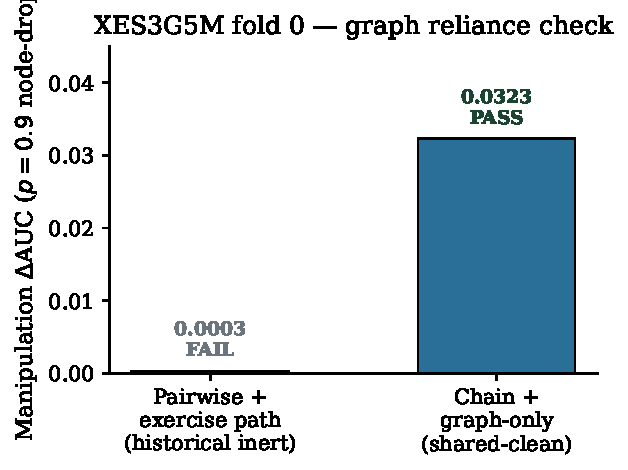
\includegraphics[width=0.92\columnwidth]{figures/fig_manipulation_sweep.pdf}
\caption{Manipulation-check $\Delta$AUC on XES3G5M fold~0 under $p{=}0.9$
node-drop. The right bar is the shared-clean evaluator
($\Delta$AUC$=0.0323$; Table~\ref{tab:manipulation}). The left bar is a
historical graph-inert path ($\Delta$AUC$\approx 0.0003$) and is
\emph{not} that evaluator. The dashed line at $0.003$ is an
\emph{illustrative} floor ($\approx$10$\times$ the graph-inert noise),
not a formal statistical cutoff from \cite{daominh2026p0}.}
\label{fig:manipulation-sweep}
\end{figure}

\FloatBarrier

\section{Hyperparameters for Table~\ref{tab:auc-xes3g5m}}
\label{app:hparams}
Table~\ref{tab:hparams} records, for each model in
Table~\ref{tab:auc-xes3g5m}, which knobs were searched, which value was
used, and how many distinct configurations were tried
\cite{pineau2021repro}. We do not claim a matched \emph{tuning} budget.
The tracer architecture was selected from a validation ablation
ladder---incidence on/off, three $\Delta t$
injection sites, and the Table~\ref{tab:negative-knowledge}
diagnostics---whereas each baseline used a single inherited
hyperparameter vector. That asymmetry favours the DH$^2$ arms in
configuration search, not the baselines.

\begin{table}[t]
\caption{Training recipes for every model in Table~\ref{tab:auc-xes3g5m}
and Table~\ref{tab:auc-inherited},
including Zero$+\Delta t$ (same optimiser as QKC-T; incidence zeroed).
``Configs tried'' counts distinct hyperparameter vectors, not seeds.
The tracer \emph{architecture} was chosen from a pre-specified ablation
ladder (Table~\ref{tab:negative-knowledge} plus Q$\leftarrow$KC and three
$\Delta t$ injection sites); its \emph{optimiser} recipe is a single
vector. GIKT/AKT/\textit{simpleKT}/DKT/DGEKT each used one inherited
\textsc{pyKT} vector \cite{liu2022pykt}. AKT and \textit{simpleKT} were
not retuned when $L$ moved from P0's 200 to 400. GIKT seed~42 (log
\texttt{C\_gikt\_clean\_L400\_e30b16}) restored best valid AUC at epoch~8
and stopped by epoch~13 under patience~5 (cap~30).}
\label{tab:hparams}
\centering
\scriptsize
\setlength{\tabcolsep}{3pt}
\begin{tabularx}{\textwidth}{@{}lXlXX@{}}
\toprule
Model & Parameter & Range searched & Selected & How chosen ($n$ configs) \\
\midrule
QKC-T / Zero$+\Delta t$ & architecture & ablation ladder & LSTM; Zero$+\Delta t$ zeros incidence & pre-specified gate \\
QKC-T / Zero$+\Delta t$ & batch / epochs / lr / $L$ / patience & --- & 16 / 30 / $10^{-3}$ / 400 / 5 & one recipe $\times$ 5 seeds \\
GIKT & batch / epochs / patience / $L$ & --- & 16 / 30 / 5 / 400 & match DH$^2$ training envelope ($n{=}1$) \\
GIKT & remaining pyKT hparams & none & P0/pyKT defaults & inherited ($n{=}1$) \\
AKT & $L$ & $\{400\}$ override & 400 & L matched; other hparams inherited ($n{=}1$) \\
AKT & lr / dropout / d\_model & none at $L{=}400$ & P0/pyKT defaults & inherited from $L{=}200$ recipe \\
\textit{simpleKT} & $L$ / other hparams & $\{400\}$ override & 400 + P0 defaults & inherited ($n{=}1$, 5 seeds) \\
DKT, DGEKT & $L$ / other hparams & $\{400\}$ override & 400 + P0 defaults & inherited, contextual ($n{=}1$, 5 seeds) \\
\bottomrule
\end{tabularx}
\end{table}

\begin{table}[H]
\caption{Inherited LSTM / dynamic-graph baselines on XES3G5M fold~0
($L{=}400$), moved out of Table~\ref{tab:auc-xes3g5m}. Five-seed
test-only mean $\pm$ sample SD on the pyKT intersection
($n{=}1{,}093{,}720$); contextual location rows, not tuning-matched
claims (Section~\ref{sec:baselines-reuse}).}
\label{tab:auc-inherited}
\centering
\footnotesize
\begin{tabular}{@{}lcc@{}}
\toprule
Model & Test-only AUC & Seeds \\
\midrule
DKT ($L{=}400$; inherited) & $0.8009{\pm}0.0002$ & 5 \\
DGEKT ($L{=}400$; inherited, contextual) & $0.7850{\pm}0.0001$ & 5 \\
\bottomrule
\end{tabular}
\end{table}


\section{Protocol residual and KC expansion}
\label{app:protocol-residual}
Table~\ref{tab:protocol-residual} records the residual between scoring
every exported KC-row and scoring the masked remainder
($+0.0101$ on QKC-T fold~0; $+0.0094$/$+0.0091$ on folds~1--2).

\begin{table}[H]
\caption{Repeat-mask residual on stored checkpoints (no new training).
P0-protocol scores every exported KC-row; clean masks repeat-row
targets. The QKC-T drop is the pyKT repeat-format effect
\cite{liu2022pykt}, not an attempt-level collapse. The no-$\Delta t$
row uses \texttt{window-mode last} and does not isolate the time
branch.}
\label{tab:protocol-residual}
\centering
\footnotesize
\begin{tabular}{@{}llrrr@{}}
\toprule
Checkpoint & Window & P0-protocol & Clean & Residual \\
\midrule
QKC-T fold~0 & chunked & 0.8397 & 0.8296 & $+0.0101$ \\
QKC-T fold~1 & chunked & 0.8392 & 0.8298 & $+0.0094$ \\
QKC-T fold~2 & chunked & 0.8382 & 0.8291 & $+0.0091$ \\
Q$\leftarrow$KC, no $\Delta t$ (window last) & last & 0.8236 & 0.8242 & $-0.0007$ \\
\bottomrule
\end{tabular}
\end{table}


A no-$\Delta t$ Q$\leftarrow$KC residual of $-0.0007$ used
\texttt{window-mode last} and a different $L$ budget: it does not
isolate the time branch from the window rule.
On the fold-0 test export every repeat row has raw
$\log(1{+}\Delta t){=}0$ ($183{,}741$ rows; $14.4\%$ of unchunked
P0-protocol targets, not of the $n{=}1{,}093{,}755$ scored set).
Because $f(0)=b$, that is a zero feature, not a proven zero hidden
state. The $6{,}413{,}353$ KC-expanded rows versus $5{,}549{,}635$
recorded attempts in \cite{liu2023xes3g5m} is the same expansion pyKT
warns about. The retrain uses the shared masking rules; it is not a
claim that we discovered KC-level row repeats.

\section{Learner-resampled bootstrap on one checkpoint pair}
\label{app:bootstrap}
Table~\ref{tab:bootstrap-qkct} records a learner-resampled diagnostic
used in Section~\ref{sec:time-result}. It
resamples 3614 learners that appear on both sides of each contrast; it
does not use the $1{,}093{,}718$-row occurrence join, is not event-aligned,
and is not a five-seed CI.

% From results/tables/b10_bootstrap_qkct_vs_{gikt,akt,simplekt}.csv
\begin{table}[H]
\caption{Learner-resampled bootstrap on one canonical fold-0 checkpoint
pair (1000 resamples of 3614 learners present on both sides). This is a
diagnostic of learner sampling, not training-seed variance, not an
event-aligned pair, and not the
five-seed Zero$+\Delta t$ gap on Table~\ref{tab:auc-xes3g5m}.
QKC-T is scored on
native $n{=}1{,}093{,}755$ positions; pyKT counterparts on the
library intersection $n{=}1{,}093{,}720$. \textit{simpleKT} AUC
$0.8203$ is the seed-42 npz, not the five-seed mean $0.8214{\pm}0.0007$.
All three difference intervals exclude zero.}
\label{tab:bootstrap-qkct}
\centering
\footnotesize
\begin{tabular}{@{}lcccc@{}}
\toprule
Contrast & AUC QKC-T & AUC other & $\Delta$ & 95\% CI of $\Delta$ \\
\midrule
vs.\ GIKT & 0.8296 & 0.8257 & $+0.0039$ & $[+0.0035,+0.0043]$ \\
vs.\ AKT & 0.8296 & 0.8223 & $+0.0073$ & $[+0.0068,+0.0077]$ \\
vs.\ \textit{simpleKT} & 0.8296 & 0.8203 & $+0.0093$ & $[+0.0088,+0.0098]$ \\
\bottomrule
\end{tabular}
\end{table}

\FloatBarrier


\bibliographystyle{elsarticle-num}
\bibliography{references}

\end{document}
